Les petites barres sur les diagrammes de Gantt (Figure \ref{gantt} et suivantes) correspondent aux différentes réunions que l'on a eu, suivies des noms des participants. Les plus grandes correspondent quant à elles aux tâches effectuées. Il y en a peu pour le moment car la phase de compréhension et d'installation des composants a été relativement longue.

\newpage
\begin{figure}
	\begin{center}
		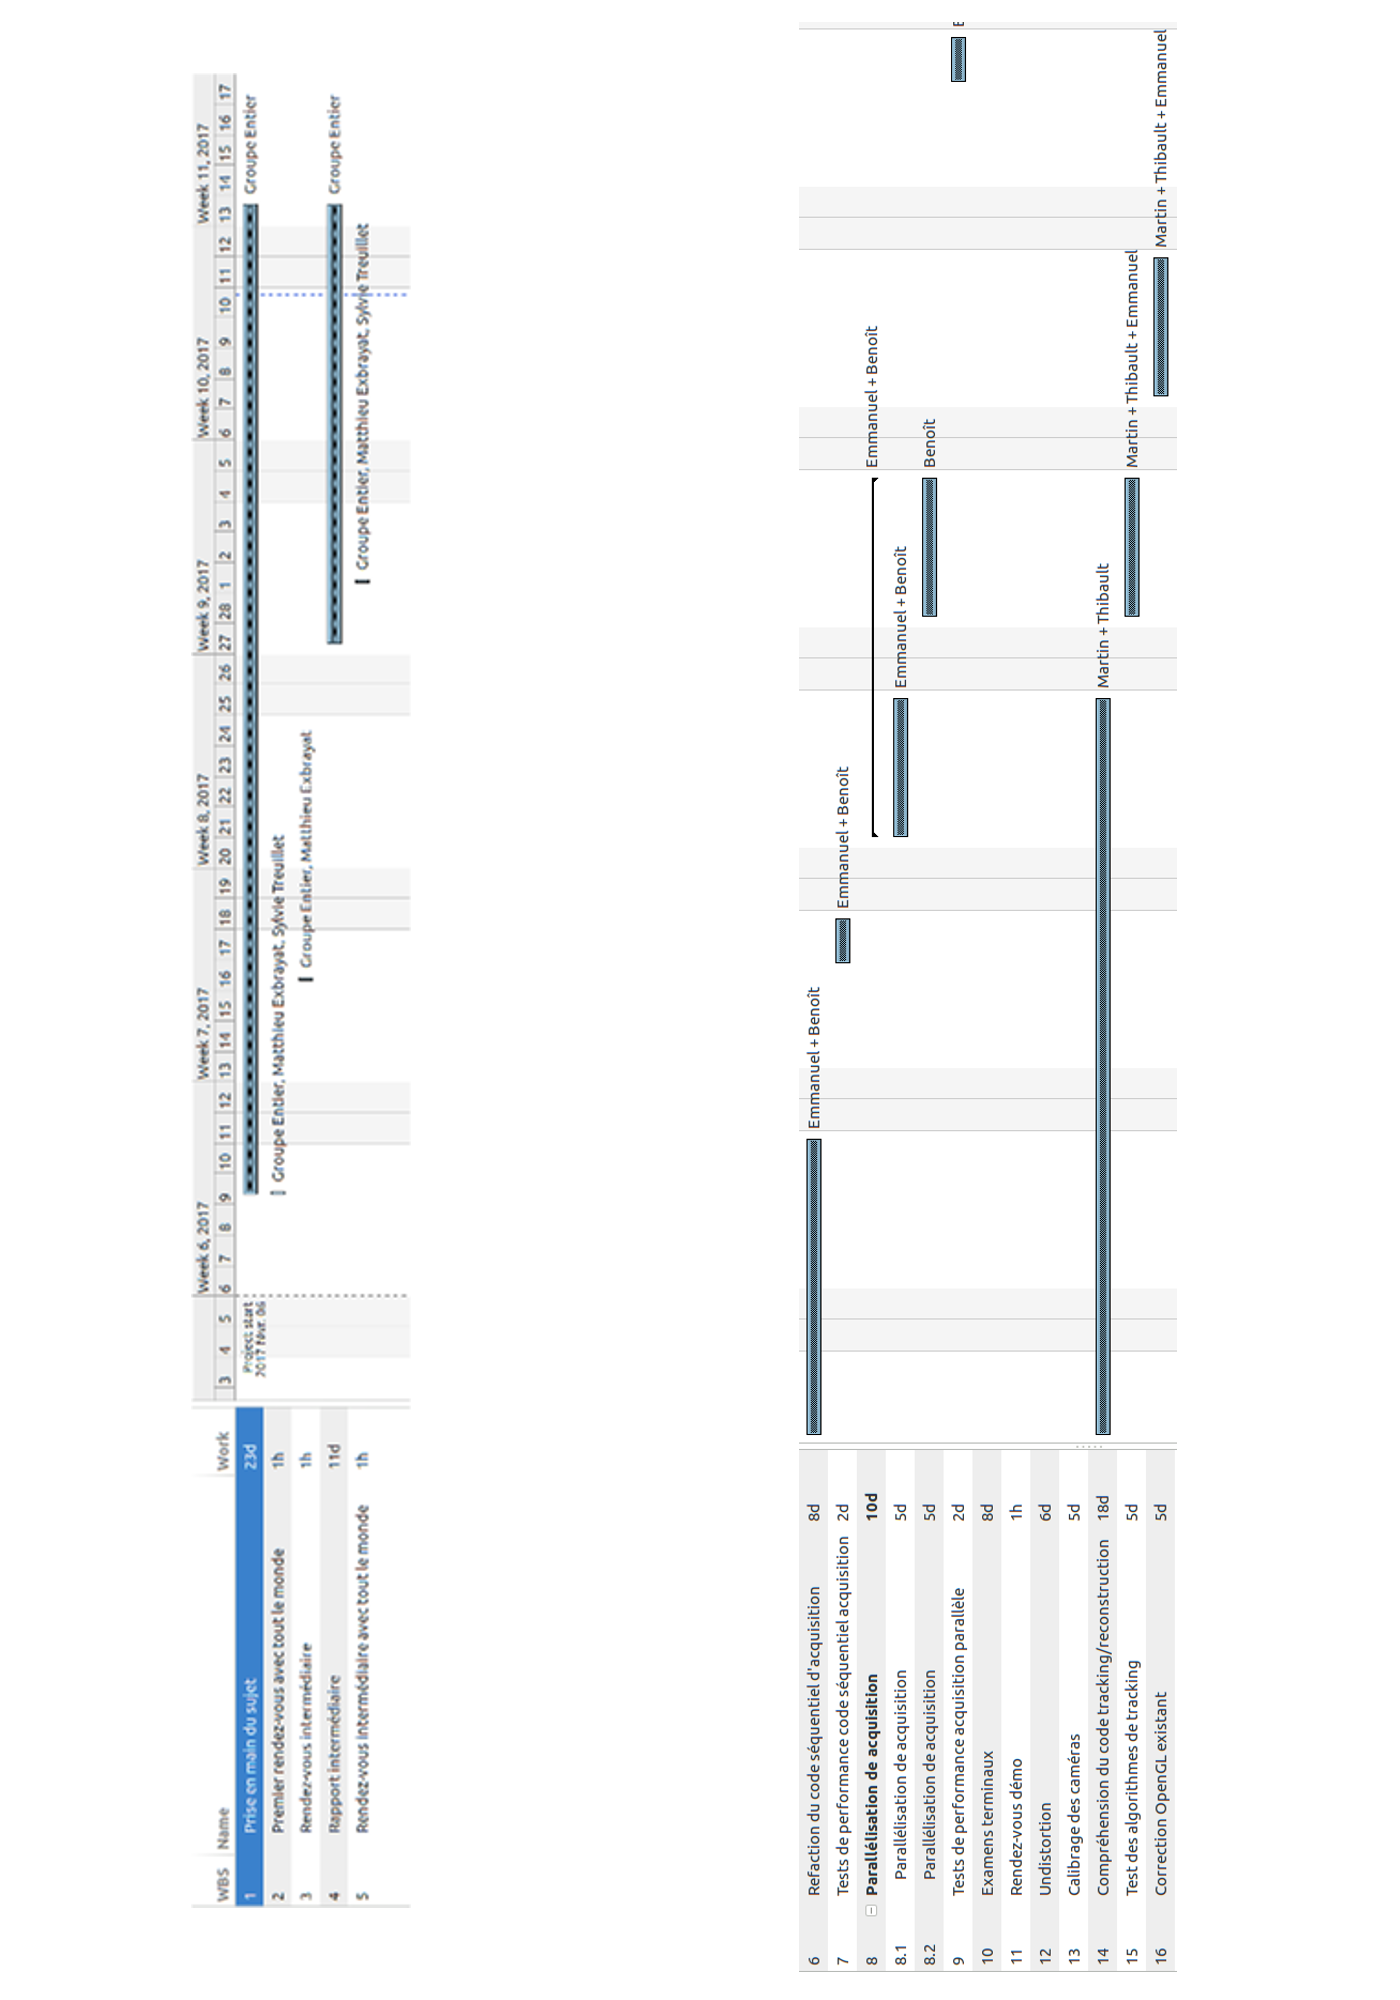
\includegraphics[scale=0.3]{Modules/Picture/gantt_0_1}
		\caption{Diagramme de Gantt 1/2}
		\label{gantt}
	\end{center}
\end{figure}

\newpage
\begin{figure}
	\begin{center}
		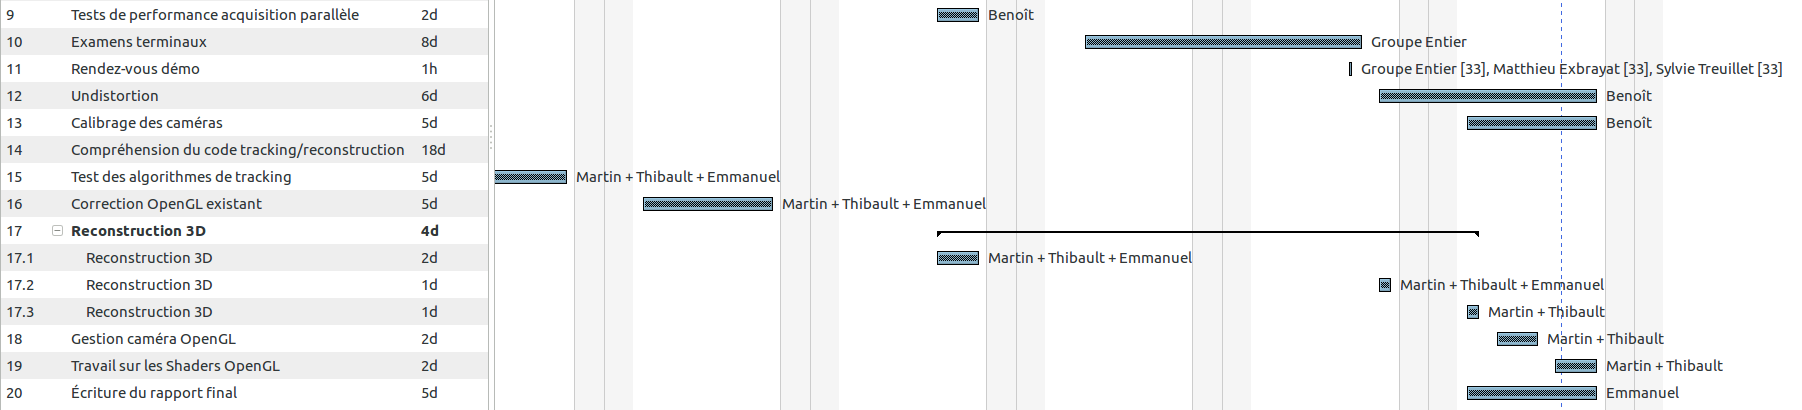
\includegraphics[scale=0.3, angle=90]{Modules/Picture/gantt_final_2}
		\caption{Diagramme de Gantt 2/2}
	\end{center}
\end{figure}

\newpage

\begin{figure}[!h]
\centering
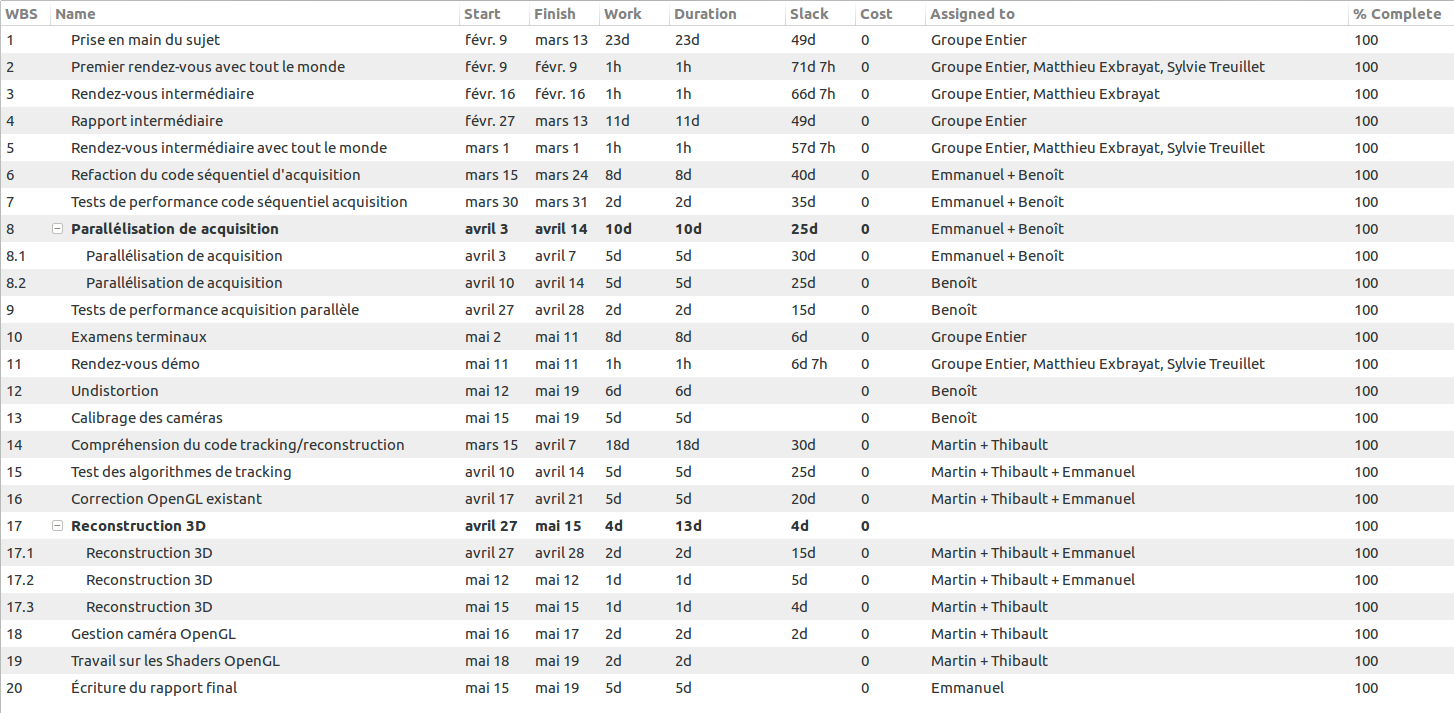
\includegraphics[scale=0.35, angle=90]{Modules/Picture/tableau_gantt_final}
\caption{Diagramme de Gantt - Total}
\label{ganttTableau}
\end{figure}

\clearpage

\newpage